\section{Remote Visual Display (RVD) Protocol}

The RVD protocol is used to communicate messages regarding mouse input, keyboard input, frame data, and clipboard
data between the
Host and the Client.\\

All messages MUST occur over the transport listed.\\

All RVD messages' first byte contain a number to indicate the message type. \\

A sequence-number is an incrementing 32-bit counter each UDP message sent, separate for Host and Client. All
messages sent over UDP MUST begin with a 4 bytes sequence-number. sequence-number is initialized
to 0 and increments once for every UDP message sent by the respective Peer. Therefore each RVD UDP message looks
like:

\begin{center}
    \begin{tabular}{|c|c|}
        \hline
        \textbf{Bytes} & \textbf{Name}   \\
        \hline
        4              & sequence-number \\
        \hline
        variable       & RVD message     \\
        \hline
    \end{tabular}
\end{center}

\subsection{Combining Messages}

In some situations, such as when a large screen change occurs or when the screen is first sent to the client,
large amounts of FrameData's may need to be sent in quick succession. Often individual FrameData's
will be much smaller than the MTU. Similar to TCP's Nagle algorithm, multiple UDP messages can be combined into a
single UDP packet as long as the total size is remains less than the MTU. Each message directly follows the
previous message with the first message directly following the sequence number. Only one sequence-number
is used:

\begin{center}
    \begin{tabular}{|c|c|}
        \hline
        \textbf{Bytes} & \textbf{Name}   \\
        \hline
        4              & sequence-number \\
        \hline
        variable       & RVD message 1   \\
        \hline
        variable       & RVD message 2   \\
        \hline
        variable       & etc.            \\
        \hline
    \end{tabular}
\end{center}

This ONLY applies to UDP messages.

\subsection{Definitions}

\begin{itemize}
    \item Host - A peer with an ID that wants to share their screen to the Client
    \item Client - A peer that wants to view and maybe control the Host's screen
    \item Display - A rectangular visual region that is shared by a Host to a Client. May or may not be
    Controllable.
    \item Controllable - A Display that accepts keyboard and mouse input from the Client.
\end{itemize}

\subsection{Handshake}

\subsubsection{ProtocolVersion - TCP}
Handshaking begins by the Host sending the client a ProtocolVersion message. This lets the Client know the
version supported by the Host.\\

The ProtocolVersion message consists of 11 bytes interpreted as a string of ASCII characters in the format
"RVD xxx.yyy" where xxx and yyy are the major and minor version numbers, padded with zeros.

\begin{center}
    Host \textrightarrow\ Client\\
    \begin{tabular}{|c|c|c|}
        \hline
        \textbf{Bytes} & \textbf{Name} & \textbf{Value}           \\
        \hline
        1              & type                 & 0                  \\
        \hline
        11             & version       & ``\texttt{RVD 001.000}'' \\
        \hline
    \end{tabular}
\end{center}

The Client replies back either \texttt{0} to indicate the version is not acceptable and that the handshake has
failed or \texttt{1} if the version is acceptable to the Client and the handshake as succeeded. If 0 is sent, all
communication MUST cease and an error SHOULD be displayed to user. A SessionEnd message should be sent by
the Client.

\begin{center}
    Client \textrightarrow\ Host\\
    \begin{tabular}{|c|c|c|}
        \hline
        \textbf{Bytes} & \textbf{Name} & \textbf{Value} \\
        \hline
        1              & type                 & 1                  \\
        \hline
        1              & ok            & 0 or 1         \\
        \hline
    \end{tabular}
\end{center}

\subsubsection{Initialization}

Once the handshake has succeeded the Host responds with a DisplayChange message.

\subsection{Control messages}
Control messages are messages that instruct the Client about changes regarding the Host.

\subsubsection{DisplayChange - TCP}
A DisplayChange message informs the Client about the available Displays. RVD supports up to 255
Displays. For each DisplayChange sent, an additional DisplayChange cannot be sent until a DisplayChangeReceived is
received by the Host.

\begin{center}
    Host \textrightarrow\ Client\\
    \begin{tabular}{|c|c|c|}
        \hline
        \textbf{Bytes} & \textbf{Name}        & \textbf{Value}     \\
        \hline
        1              & type                 & 2                  \\
        \hline
        1              & clipboard-readable   & 0 or 1             \\
        \hline
        1              & number-of-displays   & 0 - 255            \\
        \hline
        variable       & displays-information & DisplayInformation \\
        \hline
    \end{tabular}
\end{center}

Each Display has an associated DisplayInformation. displays-information contains
number-of-displays DisplayInformations. A DisplayInformation is defined below:

\begin{center}
    \begin{tabular}{|c|c|c|}
        \hline
        \textbf{Bytes}     & \textbf{Name} & \textbf{Description}                                 \\
        \hline
        1                  & display-id    &                                                      \\
        \hline
        2                  & width         & number of pixels of the width of this display        \\
        \hline
        2                  & height        & number of pixels of the width of this display        \\
        \hline
        2                  & cell-width    & number of pixels of the height of a cell in the grid \\
        \hline
        2                  & cell-height   & number of pixels of the height of a cell in the grid \\
        \hline
        1                  & access        & defined below                                        \\
        \hline
        1                  & name-length   & length of the display-name in bytes                  \\
        \hline
        \emph{name-length} & display-name  & the display name (UTF-8)                             \\
        \hline
    \end{tabular}
\end{center}

\textbf{Restrictions:}

\begin{itemize}
    \item cell-width MUST be less than width. cell-height must be less than height.\\
    \item cell-width * cell-height must be less than the MTU - headers
    \item The access byte defines what type of access is available for the display. The bits of the
    access byte are described below in little endian.
\end{itemize}


\begin{center}
    \begin{tabular}{|c|c|}
        \hline
        \textbf{Bit} & \textbf{Name}                               \\
        \hline
        0            & Flush                                       \\
        \hline
        1            & Controllable                                \\
        \hline
        2            & \multirow{6}{10em}{Reserved for future use} \\
        3            &                                             \\
        4            &                                             \\
        5            &                                             \\
        6            &                                             \\
        7            &                                             \\
        \hline
    \end{tabular}
\end{center}

If any Controllable bit is 1 and the clipboard-readable byte is set to 1, then the clipboard is
writable. The Controllable bit SHOULD be consistent throughout all displays.\\

The Flush bit indicates whether this display has changed, specifically if this display-id refers to
a different Display than the same display-id did in the previous DisplayChange message. In
initialization, this MUST always be 1 (as there is no previous DisplayChange). If the display hasn't
changed (0) then the frame data MAY be maintained. If Flush is 0, width, height MUST remain
the same as the previous DisplayChange specified for the display-id.\\


Display cell numbering is right to left, up to down, 0 indexed as seen below. If $\text{cell-width}\ \%\
\text{width} > 0$ the right column's width will be $\text{width}\ \%\ \text{cell-width}$. If $\text{height}\
\%\ \text{cell-height} > 0$ the bottom row's height will be $\text{height}\ \%\ \text{cell-height}$.

\begin{center}
    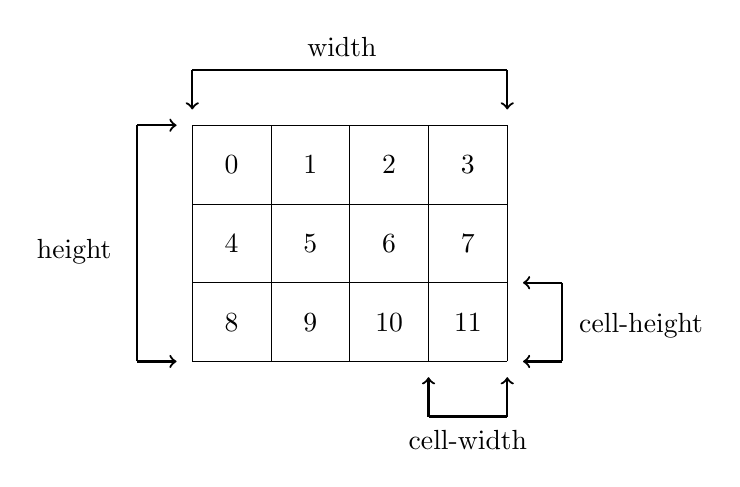
\begin{tikzpicture}
        \draw[step=1cm,black,very thin] (0,0) grid (4,3);
        \draw[thick,->] (-0.7,3) -- (-0.2,3);
        \draw[thick] (-0.7,3) -- (-0.7,0);
        \draw[thick,->] (-0.7,0) -- (-0.2,0);
        \draw (-1.5,1.4) node{height};

        \draw[thick,->] (0,3.7) -- (0,3.2);
        \draw[thick] (0,3.7) -- (4,3.7);
        \draw[thick,->] (4,3.7) -- (4,3.2);
        \draw (1.9,4) node{width};

        \draw[thick,->] (4.7,1) -- (4.2,1);
        \draw[thick] (4.7,1) -- (4.7,0);
        \draw[thick,->] (4.7,0) -- (4.2,0);
        \draw (5.7,0.45) node{cell-height};

        \draw[thick,->] (3,-0.7) -- (3,-0.2);
        \draw[thick] (3,-0.7) -- (4,-0.7);
        \draw[thick,->] (4,-0.7) -- (4,-0.2);
        \draw (3.5, -1) node{cell-width};

        \draw (0.5, 2.5) node{0};
        \draw (1.5, 2.5) node{1};
        \draw (2.5, 2.5) node{2};
        \draw (3.5, 2.5) node{3};

        \draw (0.5, 1.5) node{4};
        \draw (1.5, 1.5) node{5};
        \draw (2.5, 1.5) node{6};
        \draw (3.5, 1.5) node{7};

        \draw (0.5, 0.5) node{8};
        \draw (1.5, 0.5) node{9};
        \draw (2.5, 0.5) node{10};
        \draw (3.5, 0.5) node{11};
    \end{tikzpicture}
\end{center}

\subsubsection{DisplayChangeReceived - TCP}

The DisplayChangeReceived message is sent in reply after receiving a DisplayChange message. It
indicates to the Host they may start sending FrameData referencing the new DisplayInformation in
the most recent DisplayChange.

\begin{center}
    Client \textrightarrow\ Host\\
    \begin{tabular}{|c|c|c|}
        \hline
        \textbf{Bytes} & \textbf{Name} & \textbf{Value} \\
        \hline
        1              & type          & 3              \\
        \hline
    \end{tabular}
\end{center}

\subsubsection{MouseLocation - TCP/UDP}

The \emph{MouseLocation} message send information about where the mouse is currently on the screen.
The Host sends this information periodically throughout the session.
The Host SHOULD send a \emph{MouseLocation} update when mouse input is received from the Host's system or in
reply when it receives a \emph{MouseInput}.\\

Each shared Display has its own pointer.
Each pointer has a visibility state of visible or hidden.
Visible pointers are drawn by the Client while hidden pointers are not.
Displays begin with a hidden pointer.
When a \emph{MouseLocation} message is received, the pointer for the Display (specified by the display-id field) is made visible.
When a \emph{MouseHidden} message is received, the pointer for the Display is made hidden.

\begin{center}
    Host \textrightarrow\ Client\\
    \begin{tabular}{|c|c|c|c|}
        \hline
        \textbf{Bytes} & \textbf{Name} & \textbf{Value} & \textbf{Description}      \\
        \hline
        1              & type          & 4              &                           \\
        \hline
        1              & display-id    & 0-255          &                           \\
        \hline
        2              & x-location    &                & x coordinate of the mouse \\
        \hline
        2              & y-location    &                & y coordinate of the mouse \\
        \hline
    \end{tabular}
\end{center}

\subsubsection{MouseHidden - TCP/UDP}

\begin{center}
    Host \textrightarrow\ Client\\
    \begin{tabular}{|c|c|c|c|}
        \hline
        \textbf{Bytes} & \textbf{Name} & \textbf{Value} & \textbf{Description}      \\
        \hline
        1              & type          & 5              &                           \\
        \hline
        1              & display-id    & 0-255          &                           \\
        \hline
    \end{tabular}
\end{center}

\subsection{Input}

Input messages (including \emph{MouseLocation}) may be sent over TCP or UDP. TCP is preferred in most situations.
However, in situations where speed is prioritized over the guarantees TCP provides (such as gaming), UDP can be
used.

\subsubsection{MouseInput - TCP/UDP}

\begin{center}
    Client \textrightarrow\ Host\\
    \begin{tabular}{|c|c|c|c|}
        \hline
        \textbf{Bytes} & \textbf{Name} & \textbf{Value} & \textbf{Description}      \\
        \hline
        1              & type          & 6              &                           \\
        \hline
        1              & display-id    & 0-255          &                           \\
        \hline
        2              & x-position    &                & x coordinate of the mouse \\
        \hline
        2              & y-position    &                & y coordinate of the mouse \\
        \hline
        1              & button-mask-delta   &                & described below           \\
        \hline
        1              & button-mask-state   &                & described below           \\
        \hline
    \end{tabular}
\end{center}

%  https://github.com/rfbproto/rfbproto/blob/master/rfbproto.rst#pointerevent %
Indicates either pointer movement or a pointer button press or release. The pointer is now at (x-position,
y-position), and the current state of buttons 1 to 8 are represented by bits 0 to 7 of button-mask respectively,
0 meaning up, 1 meaning down (pressed).\\

On a conventional mouse, buttons 1, 2 and 3 correspond to the left, middle and right buttons on the mouse. On a
wheel mouse, each step of the wheel is represented by a press and release of a certain button. Button 4 means up,
button 5 means down, button 6 means left and button 7 means right.\\

button-mask-delta indicates which mouse buttons have state updates (1 indicates a state update). button-mask-state have the actual up or down state. Only state updates for buttons indicated by button-mask-delta should be considered.

\subsubsection{KeyInput - TCP/UDP}

The \emph{KeyInput} event sends key presses or releases.

\begin{center}
    Client \textrightarrow\ Host\\
    \begin{tabular}{|c|c|c|c|}
        \hline
        \textbf{Bytes} & \textbf{Name} & \textbf{Value} & \textbf{Description}                                 \\
        \hline
        1              & type          & 7              &                                                      \\
        \hline
        1              & down-flag     & 0 or 1         & indicates whether the key is now pressed or released \\
        \hline
        4              & key           &                & "keysym"                                             \\
        \hline
    \end{tabular}
\end{center}

Details can be found at the \href{https://github.com/rfbproto/rfbproto/blob/master/rfbproto.rst#keyevent}{RFB Spec}

\subsection{Clipboard}

\subsubsection{ClipboardRequest - TCP}

Used to check if a clipboard type exists on the Host.

\begin{center}
    Client \textrightarrow\ Host\\
    \begin{tabular}{|c|c|c|}
        \hline
        \textbf{Bytes}   & \textbf{Name}    & \textbf{Value} \\
        \hline
        1                & type             & 8              \\
        \hline
        1                & clipboard-type   &                \\
        \hline
        \multicolumn{3}{|c|}{\textbf{Below only if clipboard-type's first bit is 1} } \\
        \hline
        1                & type-name-length &                \\
        \hline
        type-name-length & type-name        &                \\
        \hline
    \end{tabular}
\end{center}

clipboard-type first bit (MSB) indicates whether this request is for a default type (\texttt{0}) or a custom type
(\texttt{1}). clipboard-type's second bit (second MSB) indicates whether this request is a exists request (\texttt{0}) or a
content request(\texttt{1}). An exists request is for checking whether the type exists but does not return content. A
content request returns content if it exists. The remaining bits indicate the default type if the request is for a
default type. Otherwise they MUST be 0.\\

clipboard-type's remaining bits referring to the following default types:

\begin{center}
    \begin{tabular}{|c|c|}
        \hline
        \textbf{Value} & \textbf{Description} \\
        \hline
        0              & text                 \\
        \hline
        1              & text                 \\
        \hline
        2              & rtf                  \\
        \hline
        3              & html                 \\
        \hline
        4              & file-pointer         \\
        \hline
    \end{tabular}
\end{center}

\subsubsection{ClipboardNotification- TCP}

Notifies a Peer of a clipboard update. The receiving Peer should update their clipboard.

\begin{center}
    Host $\leftrightarrow$ Client\\
    \begin{tabular}{|c|c|c|}
        \hline
        \textbf{Bytes}        & \textbf{Name}    & \textbf{Value}   \\
        \hline
        1                     & type             & 9                \\
        \hline
        1                     & clipboard-type   &                  \\
        \hline
        \multicolumn{3}{|c|}{\textbf{Below only if clipboard-type's first bit is 1} } \\
        \hline
        1                     & type-name-length &                  \\
        \hline
        type-name-length      & type-name        &                  \\
        \hline
        \multicolumn{3}{|c|}{\textbf{Below only if clipboard-type's second bit is 1} } \\
        3                     & content-length   &                  \\
        \hline
        \emph{content-length} & data             & zlib'ed raw data \\
        \hline
    \end{tabular}
\end{center}


clipboard-type, type-name-length, and type-name MUST match a request if the notification is in response. If
clipboard-readable is 0 and a Host receives a ClipboardRequest, it MUST be ignored. If no Display is Controllable or
clipboard-readable is 0 and a Host receives a ClipboardNotification, it MUST be ignored.\\

content-length -  the length of the content  (maximum $2^{24}$ bytes or ~16MB )\\

\subsection{FrameData - UDP}
The \emph{FrameData} message contains an update of a particular cell on a particular \emph{Display}.

\begin{center}
    Host \textrightarrow Client\\
    \begin{tabular}{|c|c|c|}
        \hline
        \textbf{Bytes} & \textbf{Name} & \textbf{Value} \\
        \hline
        1              & type          & 10             \\
        \hline
        4              & frame-number  &                \\
        \hline
        1              & display-id    & 0-255          \\
        \hline
        2              & cell-number   &                \\
        \hline
        2              & size          &                \\
        \hline
        \emph{size}    & data          &                \\
        \hline
    \end{tabular}
\end{center}

\emph{frame-number} is a 32 bit counter, initialized with 0 at the beginning of the protocol, and incremented once
from \emph{FrameData} message sent.

\emph{data} contains raw RGB pixel data of the updated cell.

\subsection{Congestion}

When sending messages over a network the network may become congested to avoid congesting the network further RVD
implements a congestion detection and congestion control mechanism. RVD uses Additive increase/multiplicative
decrease or AIMD to control the \emph{OutputMaximum} which is the maximum messages allowed per
\emph{CongestionWindow}.